\chapter{Uczenie modelu detekcji choroby Alzheimera oraz jego wykorzystanie}

Demencja różnych stadiów bardzo często jest powiązana z~znaczącymi, widocznymi zmianami struktury mózgowej, które można wykryć na przykład na obrazach rezonansu magnetycznego.
W tej pracy chcę przedstawić możliwości wykorzystania bibliotek uczenia maszynowego w~środowisku \emph{.NET} w~celu uczenia oraz późniejszego wykorzystania modelu głębokiej sieci neuronowej do detekcji choroby Alzheimera oraz stopnia demencji na obrazach rezonansu magnetycznego mózgów pacjentów, a~także postaram się je porównać między sobą oraz z~istniejącymi rozwiązaniami także spoza środowiska \emph{.NET}.

\section{Kod źródłowy}
\label{sec:source-code}

Kod wszystkich projektów czy narzędzi, które zostały wykorzystane w~tej pracy bezpośrednio lub pośrednio, jest dostępny w~archiwalnym repozytorium na portalu GitHub pod adresem \url{https://github.com/mmosiur/morus2023detection}.
Znajdują się tam też wytrenowane modele oraz wygenerowane wyniki, które zostały przedstawione w~tej pracy.

\section{Zbiór danych}
\label{sec:dataset}

Wykorzystany zbiór pochodzi z~platformy Kaggle (udostępniony jest pod adresem \url{kaggle.com/datasets/tourist55/alzheimers-dataset-4-class-of-images}, zapewniony na podstawie licencji \emph{Open Data Commons Open Database License} (\emph{ODbL}) wersji $1.0$) \cite{kaggle-alzheimers-dataset}.
Jest wstępnie podzielony na zbiór treningowy oraz testowy w~celu zapewnienia powtarzalności i~porównywalności wyników uzyskanych z~użyciem różnych narzędzi i~z różnych źródeł.
Zawiera on zestaw obrazów uzyskanych z~badań rezonansem magnetycznym (MRI), których celem jest analiza i~diagnoza otępienia spowodowanego chorobą Alzheimera.
Obrazy te są dwuwymiarowym wycinkiem trójwymiarowego skanu rezonansu magnetycznego mózgu, który najlepiej obrazuje strukturę mózgu i~potencjalne zmiany chorobowe.
Mają wymiary $208 \times 176$ pikseli -- wystarczająco duże, aby widoczne były nawet drobne detale, ale na tyle małe, aby były możliwe do przetworzenia przez mniejsze sieci neuronowe a~także umożliwiły ich znacznie szybsze szkolenie.

Zbiór danych składa się z~czterech kategorii obrazów, zarówno w~zbiorze treningowym, jak i~testowym:

\begin{itemize}

  \item
        Brak demencji (\emph{Non Demented}) -- ta kategoria zawiera obrazy mózgów osób niebędących dotkniętymi demencją.
        W~zbiorze treningowym znajduje się 2560 obrazów, a~w zbiorze testowym 640 obrazów, co daje sumarycznie 3200 zdjęć z~tej kategorii.

  \item
        Bardzo łagodna demencja (\emph{Very Mild Demented}) -- zbiór ten obejmuje obrazy osób z~bardzo łagodnym stopniem demencji.
        W~zbiorze treningowym znajduje się 1792 obrazy, a~w zbiorze testowym 448 obrazów, co daje łącznie 2240 obrazów z~tej kategorii.

  \item
        Łagodna demencja (\emph{Mild Demented}) -- ten zbiór zawiera obrazy mózgów pacjentów cierpiących na łagodne otępienie związanego z~chorobą Alzheimera.
        W~zbiorze treningowym znajduje się 717 obrazów, a~w zbiorze testowym 179 obrazów, co daje łączną sumę 896 obrazów z~tej kategorii.

  \item
        Umiarkowana demencja (\emph{Moderate Demented}) -- ta kategoria obejmuje obrazy mózgów pacjentów już z~wyższym stopniem demencji związanym z~chorobą Alzheimera.
        W~zbiorze treningowym znajduje się 52 obrazy, a~w zbiorze testowym 12 obrazów, co daje łącznie 64 obrazy z~tej kategorii.

\end{itemize}

\begin{figure}[ht]
  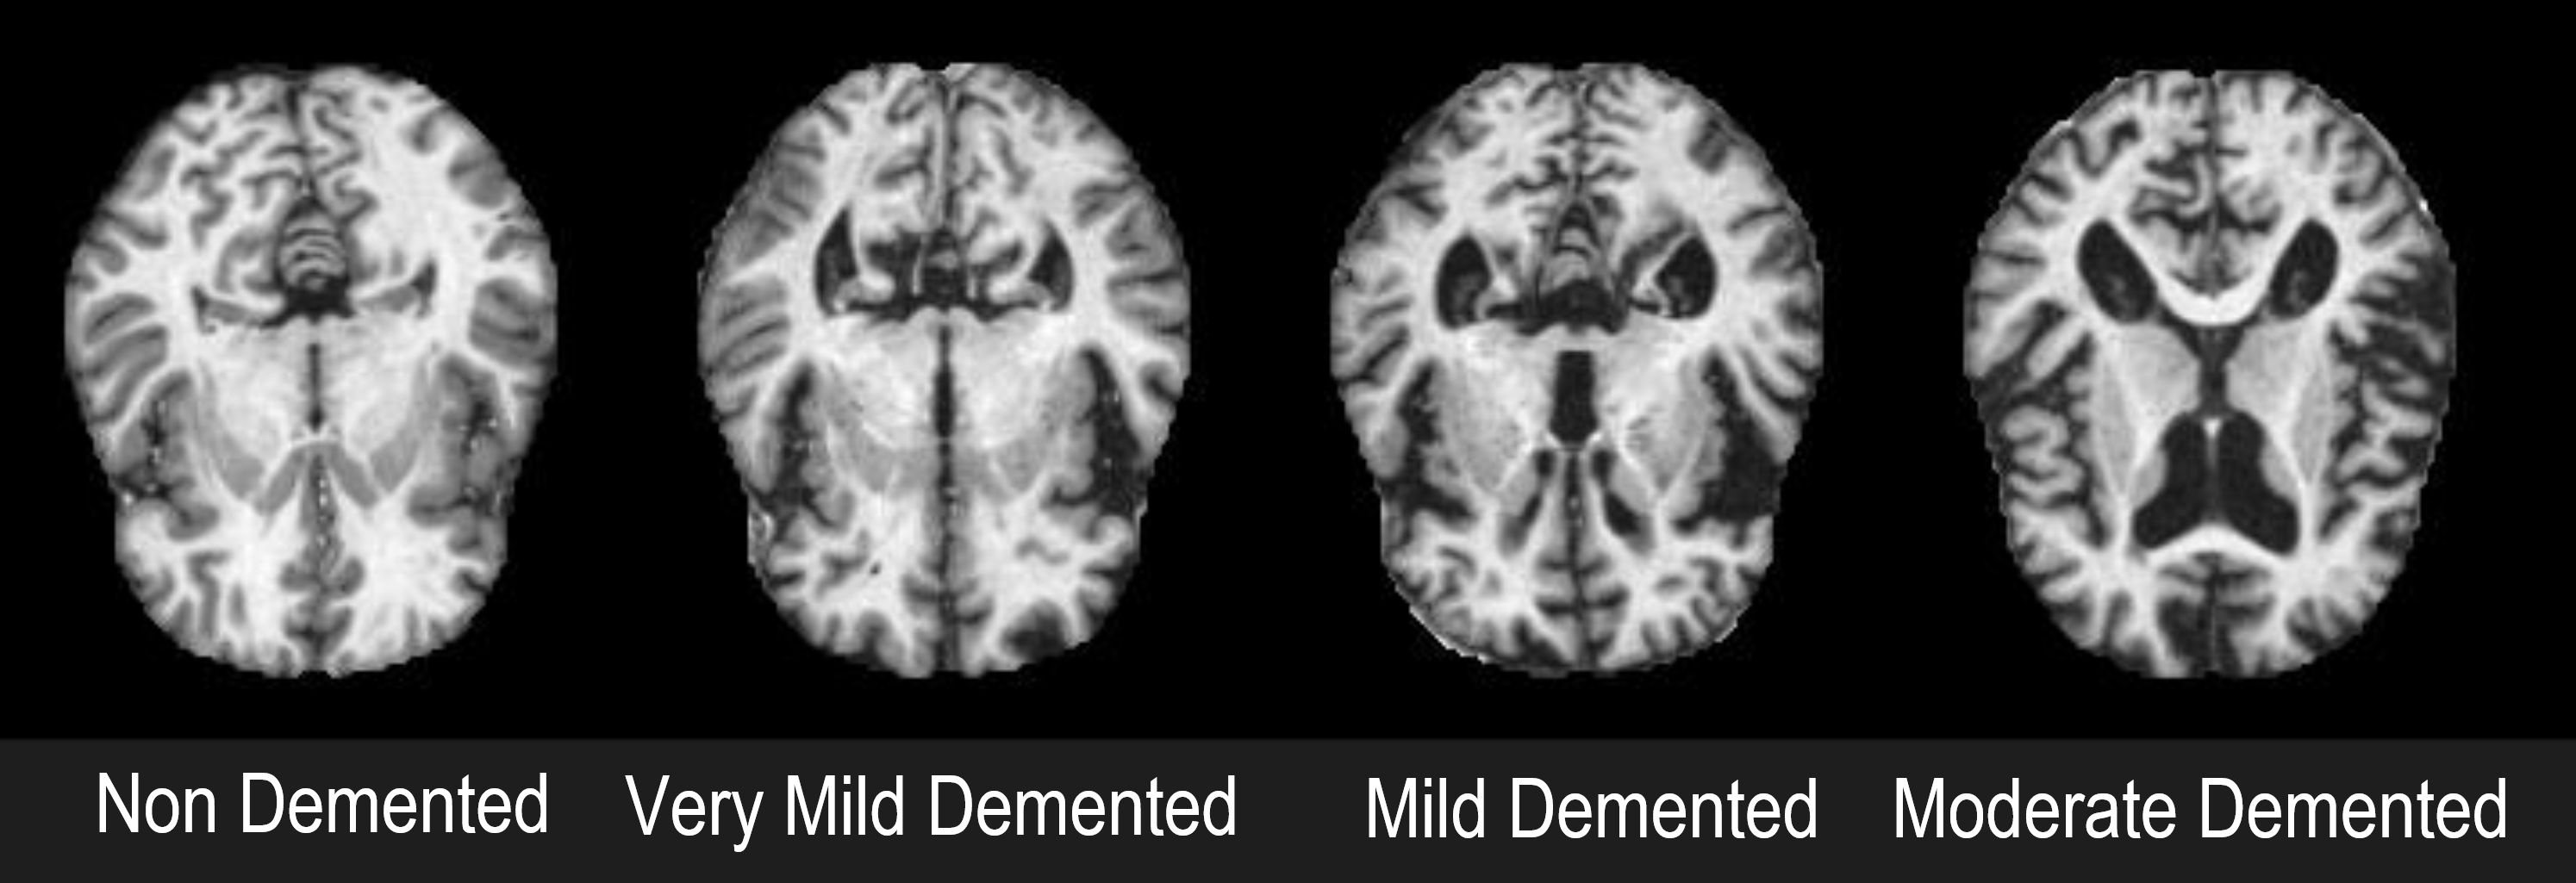
\includegraphics[width=\textwidth]{dataset-image-examples}
  \caption[Zestawienie przykładowych obrazów z~każdej kategorii zbioru danych]{Zestawienie przykładowych obrazów z~każdej kategorii zbioru danych \cite{kaggle-alzheimers-dataset}, gdzie przedstawione od lewej są: obraz mózgu osoby bez demencji, obraz mózgu osoby z~bardzo lekką demencją, obraz mózgu osoby z~lekką demencją o~podłożach w~chorobie Alzheimera oraz obraz mózgu osoby z~umiarkowaną demencją chorą na Alzheimera.}
  \label{fig:dataset-image-examples}
\end{figure}

Przykłady obrazów z~poszczególnych kategorii przedstawione są na \hyperref[fig:dataset-image-examples]{rysunku \ref*{fig:dataset-image-examples}}.

\section{Uczenie modelu z~użyciem narzędzia ML.NET}

Oczywistym pierwszym kandydatem do podjęcia próby uczenia modelu głębokiej sieci neuronowej w~celu detekcji choroby Alzheimera jest projekt utrzymywany przez \emph{.NET Foundation} -- a~więc najbliższy natywnemu środowisku \emph{.NET} -- biblioteka \emph{ML.NET}.
Została ona szczegółowiej opisana i~scharakteryzowana w~\hyperref[sec:ml-net]{sekcji \ref*{sec:ml-net}}.
I warto również przypomnieć, że pozwala ona na budowanie modeli uczenia maszynowego na dwa główne sposoby -- ręczne pisanie kodu w~języku \emph{C\#} (lub dowolnego innego z~rodziny języków .NET takich jak \emph{F\#} czy \emph{Visual Basic}) z~użyciem API biblioteki \emph{ML.NET} lub z~użyciem narzędzia \emph{ML.NET Model Builder} wbudowanego w~zintegrowane środowisko programistyczne Visual Studio.
Z obu podejść skorzystałem i~zestawiłem je ze sobą w~celu porównania.

\subsection{Uczenie modelu z~wykorzystaniem własnego kodu biblioteki ML.NET}

Wykorzystanie API biblioteki ML.NET do uczenia modelu głębokiej sieci neuronowej nie wymaga skomplikowanego kodu ani podejścia.
Napisany przeze mnie projekt znajdujący się w~repozytorium opisanym w~\hyperref[sec:source-code]{sekcji \ref*{sec:source-code}} już na pierwszy rzut oka jest nieco bardziej złożony.
Wygląda on tak, ponieważ wykorzystałem możliwości języka C\# oraz podejście, przy którym bardzo dobrze się sprowadza i~wprowadziłem ustrukturyzowane podejście obiektowe.
Generuje ono nieco więcej kodu niż podejście imperatywne, jednak jest ono bardziej czytelne i~łatwiejsze do zrozumienia przy rosnącej złożoności systemu, a~także pozwala na łatwiejsze wprowadzanie zmian i~rozwijanie projektu czy wprowadzenie utworzonego rozwiązania do innego, już istniejącego systemu.

Solucja \lstinline{MLNetCustom.sln} zawiera trzy projekty: główny projekt \lstinline{MLNetCustom.csproj} napisany w~języku C\# i~zawierający faktycznie szkolenie i~wykorzystanie biblioteki \emph{ML.NET}, projekt \lstinline{Plot.fsproj} napisany w~języku F\# zawierający kod funkcji wykorzystujących bibliotekę \emph{Plotly.NET} do wygenerowania wykresów na bazie przekazanych metryk, oraz projekt \lstinline{PlotGenerator.csproj} wystawiający API w~postaci klas opakowujących funkcje generowania wykresów z~projektu F\# \lstinline{Plot.fsproj}.

Przedstawia to też dobrze siłę i~możliwości platformy \emph{.NET}, gdzie jedna solucja jest modularnym tworem składającym się z~wielu bytów mogących być napisanymi w~różnych językach programowania, a~także wykorzystującymi różne biblioteki i~narzędzia w~celu jak najbardziej przejrzystego ustrukturyzowania kodu i~jego łatwiejszej rozbudowy i~utrzymania.

Skupiając się jednak na najistotniejszym projekcie \lstinline{MLNetCustom.csproj} zawierającym faktyczny kod uczenia modelu głębokiej sieci neuronowej, można zauważyć, że on także jest wewnętrznie napisany w~sposób modularny.
Wejście programu jest zdefiniowane w~postaci specjalnego skryptu w~pliku \lstinline{Program.cs}, który wykonywany jest jako ciało funkcji głównej programu.
Aby jednak zachować czytelność, są tam głównie wywoływane funkcje i~metody klas napisanych w~pozostałych plikach.

Istotnym punktem API biblioteki \emph{ML.NET} jest klasa \lstinline{MLContext}, która przechowuje globalny stan generatora liczb pseudolosowych dla całego procesu uczenia modelu, a~także udostępnia metody pomocnicze do ładowania danych, tworzenia modelu, jego uczenia i~ewaluacji.
Na nim także bazują klasy napisane w~celu enkapsulacji działań na bibliotece, w~tym klasa \lstinline{DatasetProvider}.

Obudowuje ona proces wczytywania danych wejściowych -- treningowych oraz testowych -- ze zbioru danych w~postaci opisanej w~\hyperref[sec:dataset]{sekcji \ref*{sec:dataset}}.
Udostępnia następnie wczytane dalej w~prostszej do wykorzystania postaci.
Funkcja wczytująca dane pochodząca z~tej klasy została przedstawiona poniżej:

\begin{lstlisting}[language={[Sharp]C}]
private IDataView LoadImagesFromDirectory(string directory, out DataViewSchema schema)
{
  var imagesMetadata = Directory
    .GetDirectories(directory)
    .Select(subdirectory => new { Path = subdirectory, Label = Path.GetFileName(subdirectory)! })
    .SelectMany(
      collectionSelector: dir => Directory.GetFiles(dir.Path),
      resultSelector: (dir, file) => new ImageMetadata { ImagePath = file, Label = dir.Label }
    );
  var imagesDataset = _context.Data.LoadFromEnumerable(imagesMetadata);
  schema = imagesDataset.Schema;
  imagesDataset = _context.Data.ShuffleRows(imagesDataset, _options.Seed);

  var preprocessingPipeline = _context.Transforms.Conversion.MapValueToKey(
      inputColumnName: nameof(ModelInputDefinition.Label),
      outputColumnName: nameof(ModelInputDefinition.LabelAsKey))
    .Append(_context.Transforms.LoadRawImageBytes(
      outputColumnName: nameof(ModelInputDefinition.Image),
      imageFolder: directory,
      inputColumnName: nameof(ModelInputDefinition.ImagePath)));

  return preprocessingPipeline
    .Fit(imagesDataset)
    .Transform(imagesDataset);
}
\end{lstlisting}

Dodatkowo przedstawione tutaj jest wykorzystanie ``fluent interfejsów'' pozwalających na łańcuchowe wywoływanie po sobie metod, poprawiając czytelność kodu opisanych w~\hyperref[sec:csharp]{sekcji \ref*{sec:csharp}} o~języku C\#.

Druga z~istotniejszych klas własnych to \lstinline{AlzheimerPredictionEngineTrainer}, która obudowuje sam model, proces jego uczenia oraz testowania używając instancji klasy \lstinline{DatasetProvider} jako źródła danych.
Fragment metody uczącej z~wyciętą częścią odpowiedzialną za tworzenie obiektu opcji konfigurujących proces uczenia przedstawiony jest poniżej:

\begin{lstlisting}[language={[Sharp]C}]
public void Train(Options? options = null)
{
  options ??= new();

  if (!_datasetProvider.IsDatasetLoaded)
  {
    _datasetProvider.LoadDataset();
  }

  // Building `classifierOptions` variable using `options` argument

  var trainingPipeline = _context.MulticlassClassification.Trainers.ImageClassification(classifierOptions)
    .Append(_context.Transforms.Conversion.MapKeyToValue(classifierOptions.PredictedLabelColumnName));

  _model = trainingPipeline.Fit(_datasetProvider.TrainSet);
}
\end{lstlisting}

Wycięte budowanie zmiennej \lstinline{classifierOptions} z~użyciem argumentu \lstinline{options} przekazuje tylko parametry takie jak \lstinline{Arch} ustalające wykorzystaną do szkolenia architekturę sieci transferowej (enum z~wartością \lstinline{InceptionV3}, \lstinline{MobilenetV2}, \lstinline{ResnetV2101} lub \lstinline{ResnetV250}), \lstinline{Epoch} przechowujące ilość epok uczenia, \lstinline{LearningRate} ustawiające współczynnik uczenia i~inne.

Wywołanie tej metody na utworzonym obiekcie wygląda następująco:

\begin{lstlisting}[language={[Sharp]C}]
const int epochCount = 200;
engine.Train(new()
{
  MetricsCallback = metrics =>
  {
    plotGenerator.Data.Add(metrics);
    Console.WriteLine($"Epoch {metrics.Train.Epoch+1}/{epochCount}, dataset {metrics.Train.DatasetUsed}");
  },
  Epoch = epochCount,
  Architecture = ImageClassificationTrainer.Architecture.ResnetV2101,
  LearningRateScheduler = new ExponentialLRDecay(0.01f, 20)
});
\end{lstlisting}

Na tym fragmencie widać, że do uczenia sieci wykorzystałem architekturę opartą na \emph{ResNet V2 101} i~z uczeniem o~czasie $200$ epok.
Wartości parametrów \lstinline{LearningRate} (współczynniku uczenia) czy \lstinline{BatchSize} (rozmiaru paczki danych) nie zostały zmienione i~ustalone są domyślnie na wartości odpowiednio $0.01$ i~$10$.

Uruchomiony program rozpoczynał proces uczenia modelu, z~którego dane przebiegu zostały przedstawione na \hyperref[fig:plot-mlnet-custom-training-overview]{rysunku \ref*{fig:plot-mlnet-custom-training-overview}} z~wykresem dokładności (\emph{accuracy}) oraz straty (\emph{loss}) dla danych testowych i~walidacyjnych w~trakcie uczenia.

\begin{figure}[ht]
  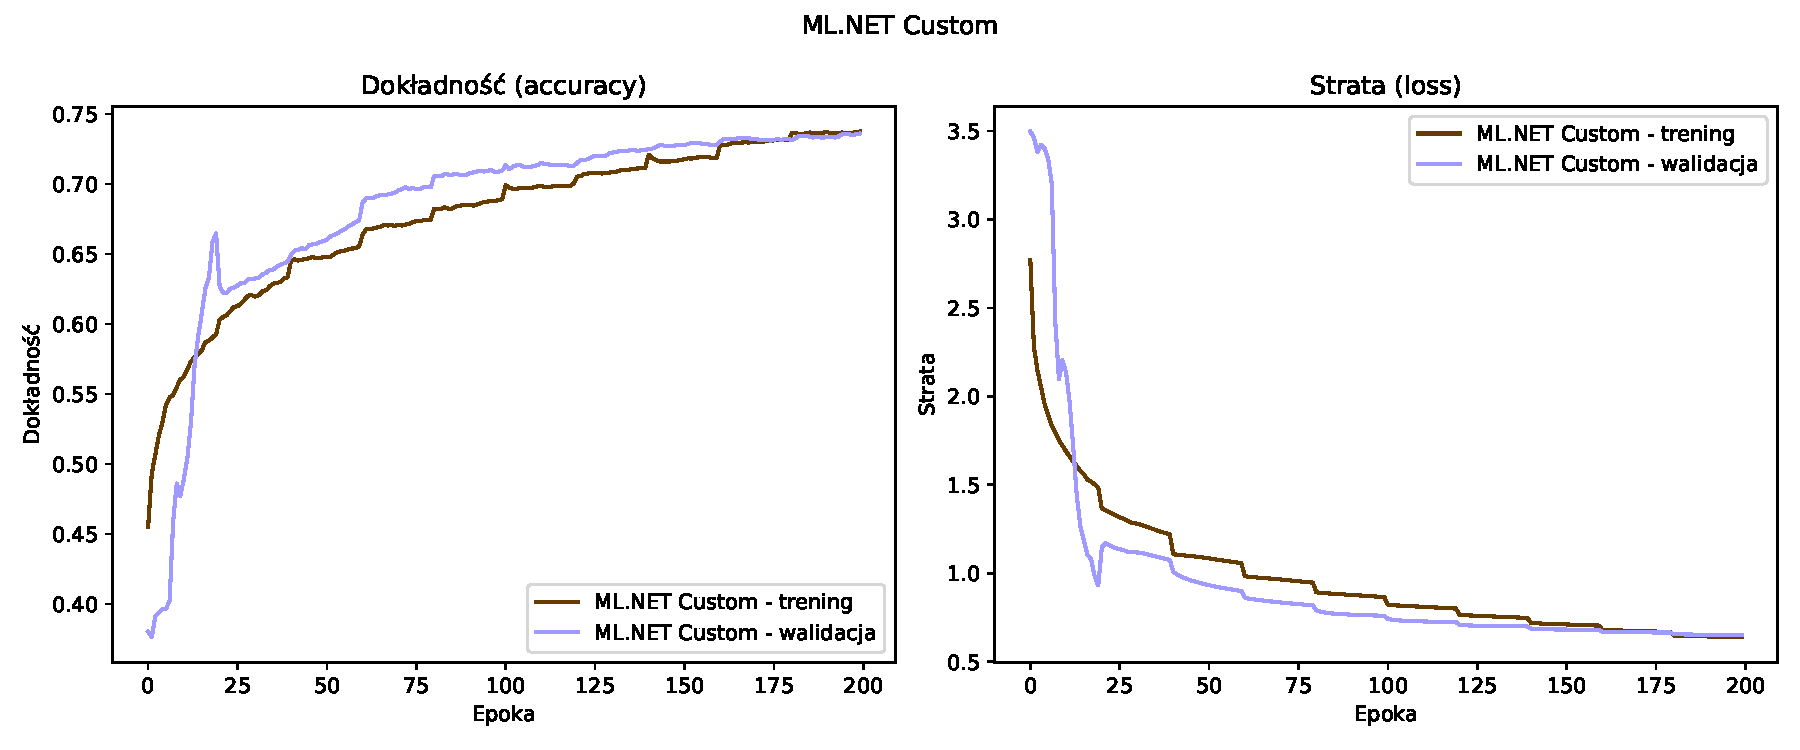
\includegraphics[width=\textwidth]{plot-mlnet-custom-training-overview}
  \caption[Wykresy statystyk modelu ML.NET Custom w~trakcie uczenia]{Wykresy dokładności (\emph{accuracy}) oraz straty (\emph{loss}) dla danych testowych i~walidacyjnych modelu \emph{ML.NET Custom} w~trakcie uczenia}
  \label{fig:plot-mlnet-custom-training-overview}
\end{figure}

Przedstawione dane pokazują, że model prawidłowo zaczął się uczyć w~rosnącą dokładnością zarówno w~zbiorze treningowym, jak i~walidacyjnym oraz podobnie malejącą stratą.
Najwyższa wartość dokładności na zbiorze treningowym wyniosła $73.7\%$, a~na zbiorze walidacyjnym $73.6\%$.

Tak nauczona sieć została natomiast później przetestowana na zbiorze testowym, który nie został użyty w~procesie uczenia, a~więc sieć widziała pojawiające się tam obrazy po raz pierwszy.
Uzyskała ona wynik dokładności $45.3\%$ -- czyli lepszy niż losowy (który dla 4~kategorii wynosiłby $0.25$), ale zdecydowanie niezadowalający, gdzie ponad połowa obrazów została źle sklasyfikowana.
Potencjalny wzrost dokładności modelu przy podniesieniu już wysokiej ilości epok byłby mało prawdopodobny, gdyż wzrost był w~końcowym etapie już znikomy i~prawdopodobnie zbliżał się moment przeuczenia sieci, a~co za tym idzie dokładność na zbiorze walidacyjnym oraz testowa zaczęłyby spadać.

\subsection{Uczenie modelu z~użyciem narzędzia ML.NET Model Builder}

Oprócz umożliwienia napisania własnego kodu wykorzystującego bezpośrednio API biblioteki, \emph{ML.NET} pozwala również na automatyczne wyszkolenie modelu i~wygenerowanie kodu na jego ponowne przeszkolenie czy wykorzystanie w~kodzie w~praktyce.
W tym celu wykorzystuje się narzędzie \emph{ML.NET Model Builder} wbudowane w~zintegrowane środowisko programistyczne Visual Studio, które w~sposób bardziej szczegółowy przedstawione zostało w~\hyperref[sec:ml-net-model-builder]{sekcji \ref*{sec:ml-net-model-builder}}.

Narzędzie to pozwala na interaktywne, graficzne wybieranie rodzaju uczenia maszynowego do przeprowadzenia, wskazania danych czy wybrania środowiska do przeprowadzenia uczenia, przedstawione między innymi na rysunkach \ref{fig:ml-net-model-builder-1-scenario} i~\ref{fig:ml-net-model-builder-2-training-data}.

W przeciwieństwie do projektu, w~którym własnoręcznie wykorzystuje się API biblioteki, \emph{ML.NET Model Builder} nie daje praktycznie żadnej możliwości konfiguracji procesu uczenia czy jakichkolwiek hiperparametrów modelu, wszystkie dane dobierane są automatycznie.

W procesie uczenia generowane są logi z~jego przebiegu, które zostały także zawarte w~repozytorium opisanym w~\hyperref[sec:source-code]{sekcji \ref*{sec:source-code}} w~solucji \lstinline{VisualStudioModelBuilder}.
ML.NET Model Builder pozwala również na wygenerowanie przykładowych projektów .NET prezentujących przykładowe wykorzystanie utworzonego, nauczonego modelu w~praktyce.
Projekty takie zostały także wygenerowane i~zawarte w~repozytorium -- \lstinline{MLModel_ConsoleApp} przedstawiający przykładową aplikację konsolową oraz \lstinline{MLModel_WebApi} przedstawiający przykładową aplikację internetową z~interfejsem REST API.
Zawarty tam również został projekt \lstinline{MLModel_Test}, który wykorzystuje API ML.NET w~celu przetestowania powstałego modelu na zbiorze testowym.

Z pliku logów wyekstrahowane zostały dane numeryczne dotyczące przebiegu uczenia modelu, które zostały przedstawione na \hyperref[fig:plot-mlnet-model-builder-training-overview]{rysunku \ref*{fig:plot-mlnet-model-builder-training-overview}} z~wykresem dokładności (\emph{accuracy}) oraz straty (\emph{loss}) dla danych testowych i~walidacyjnych w~trakcie uczenia.

\begin{figure}[ht]
  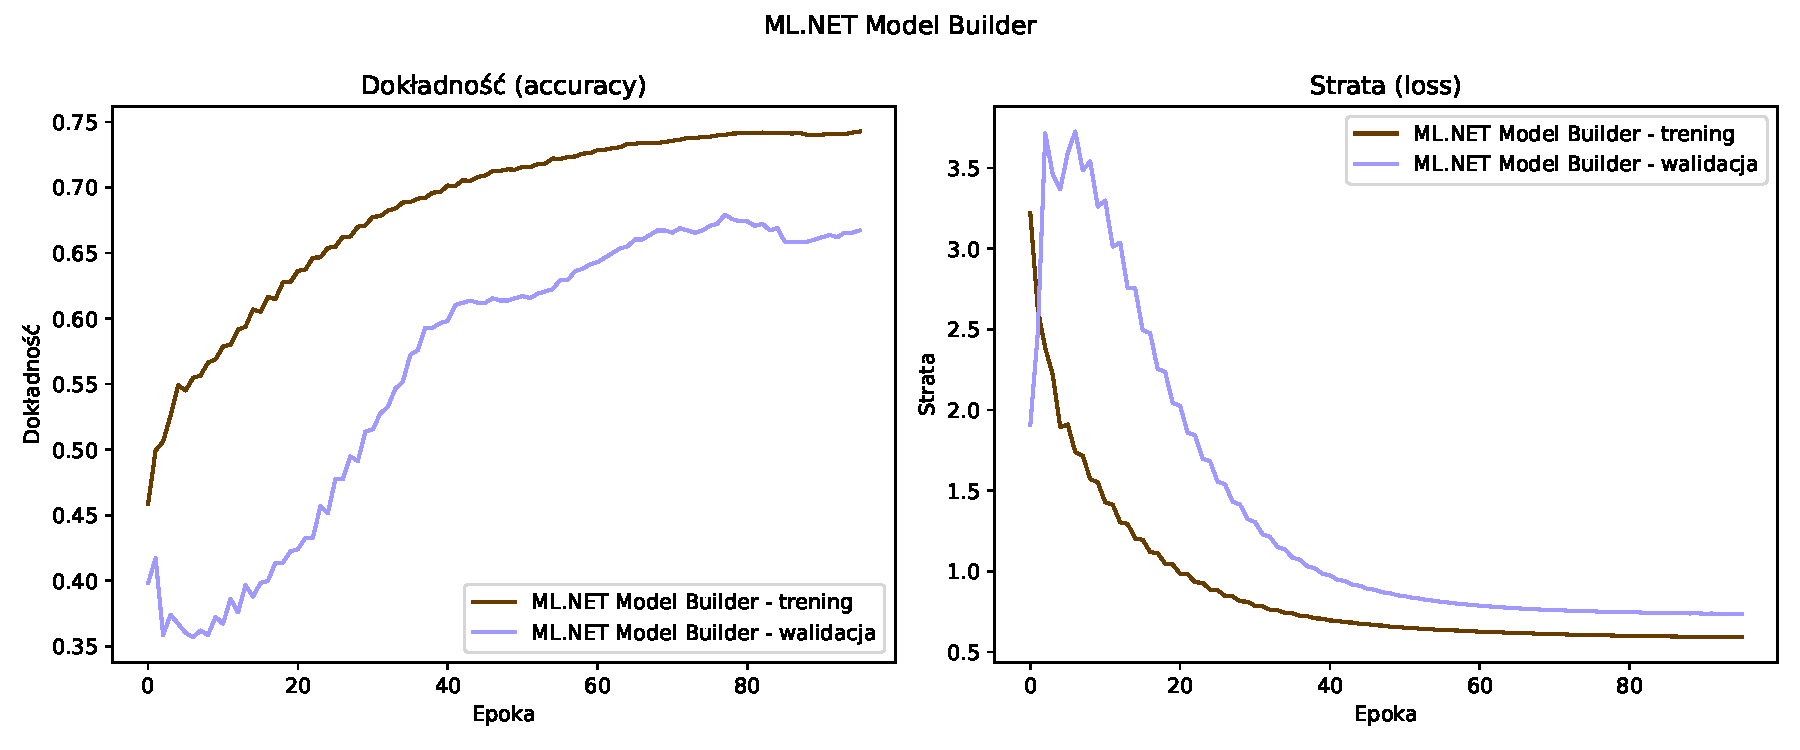
\includegraphics[width=\textwidth]{plot-mlnet-model-builder-training-overview}
  \caption[Wykresy statystyk modelu ML.NET Model Builder w~trakcie uczenia]{Wykresy dokładności (\emph{accuracy}) oraz straty (\emph{loss}) dla danych testowych i~walidacyjnych modelu \emph{ML.NET Model Builder} w~trakcie uczenia}
  \label{fig:plot-mlnet-model-builder-training-overview}
\end{figure}

Przedstawione dane pokazują, że model prawidłowo zaczął się uczyć w~rosnącą dokładnością zarówno w~zbiorze treningowym, jak i~walidacyjnym oraz podobnie malejącą stratą.
Najwyższa wartość dokładności na zbiorze treningowym wyniosła $74.0\%$, a~na zbiorze walidacyjnym $67.9\%$.
W wyniku przetestowania działania modelu na zbiorze testowym uzyskano dokładność $70.6\%$, która jest zdecydowanie lepsza niż w~przypadku własnoręcznie napisanego kodu, ale nadal niezadowalająca do zastosowań praktycznych, gdzie prawie co trzeci obraz został źle sklasyfikowany.

Zauważyć natomiast warto, że uczenie trwało $95$ epok, po czym zostało automatycznie przerwane, gdyż dalsze uczenie nie przynosiło już żadnych widocznych korzyści -- dokładność przestała rosnąć, a~strata maleć -- co wskazuje na to, że model został nauczony optymalnie i~dalsze uczenie mogłoby doprowadzić do przeuczenia sieci i~pogorszenia jej dokładności na zbiorze testowym.

\section{Uczenie niestandardowego modelu z~użyciem biblioteki TensorFlow.NET}

Alternatywą do biblioteki \emph{ML.NET} utrzymywanej przez \emph{.NET Foundation} jest biblioteka \emph{TensorFlow.NET} utrzymywana przez społeczność w~ramach projektów \emph{SciSharp}.
Pozwala ona na wydajne wykorzystanie biblioteki \emph{TensorFlow} oraz \emph{Keras} w~środowisku \emph{.NET} wystawiając połączenia do natywnego kodu \emph{TensorFlow} w~języku \emph{C}.
Sama biblioteka \emph{TensorFlow} została szczegółowiej opisana w~\hyperref[sec:tensorflow-and-keras]{sekcji \ref*{sec:tensorflow-and-keras}}, natomiast jej nakładka w~środowisku \emph{.NET} -- \emph{TensorFlow.NET} -- w~\hyperref[sec:tensorflownet]{sekcji \ref*{sec:tensorflownet}}.

W praktyce biblioteka ta ma bardzo ściśle symulować doświadczenie deweloperskie używania \emph{TensorFlow} oraz \emph{Keras} w~języku \emph{Python}.
W wyniku tego sposób używania biblioteki \emph{TensorFlow.NET} jest bardzo podobny do pierwowzoru oraz jest znacznie bardziej imperatywny w~użyciu, generując płaski, długi kod przypominający wydłużony skrypt.

W mojej implementacji modelu znajdującej się w~repozytorium opisanym w~\hyperref[sec:source-code]{sekcji \ref*{sec:source-code}} znajduje się solucja \lstinline{TensorFlowNet} oraz projekt o~tej samej nazwie, który zawiera kod uczenia modelu głębokiej sieci neuronowej do problemu badawczego.
Kod składa się z~jednego pliku \lstinline{Program.cs} zawierającego cały kod programu, w~sposób przypominający skrypt języka Python.
Widoczne to jest między innymi po sposobie wczytywania danych przedstawionym poniżej, który jest bardzo podobny do tego, który można znaleźć w~rozwiązaniach w~języku Python:

\begin{lstlisting}[language={[Sharp]C}]
var AUTOTUNE = tf.data.AUTOTUNE;
var IMAGE_SIZE = (176, 208);
var EPOCHS = 100;
var BATCH_SIZE = 16;
var class_names = new[] { "MildDemented", "ModerateDemented", "NonDemented", "VeryMildDemented" };
/// ...
var train_ds = keras.preprocessing.image_dataset_from_directory(
  directory: @"path/to/dataset",
  validation_split: 0.2f,
  subset: "training",
  class_names: class_names,
  seed: 1213,
  image_size: IMAGE_SIZE,
  batch_size: BATCH_SIZE
);
\end{lstlisting}

Jako że biblioteka ta jest nakładką na \emph{Keras}, pozwala na bardzo dużą dozę swobody konfiguracji a~także tworzenia struktury sieci neuronowej, wliczając to kolejność, ilość oraz rodzaj warstw.
Dla celów detekcji choroby Alzheimera zdecydowałem się na utworzenie dużego modelu głębokiej sieci konwolucyjnej w~sposób przedstawiony poniżej:

\begin{lstlisting}[language={[Sharp]C}]
Func<Model> build_model = () =>
{
  IEnumerable<ILayer> ConvBlock(int filters)
  {
    yield return keras.layers.Conv2D(filters, 3, activation: "relu", padding: "same");
    yield return keras.layers.Conv2D(filters, 3, activation: "relu", padding: "same");
    yield return keras.layers.BatchNormalization();
    yield return keras.layers.MaxPooling2D();
  }

  IEnumerable<ILayer> DenseBlock(int units, float dropout_rate)
  {
    yield return keras.layers.Dense(units, activation: "relu");
    yield return keras.layers.BatchNormalization();
    yield return keras.layers.Dropout(dropout_rate);
  }

  var layers = new List<ILayer>();
  layers.Add(keras.layers.InputLayer(input_shape: (IMAGE_SIZE.Item1, IMAGE_SIZE.Item2, 3)));
  layers.Add(keras.layers.Conv2D(8, 3, activation: "relu", padding: "same"));
  layers.Add(keras.layers.Conv2D(8, 3, activation: "relu", padding: "same"));
  layers.Add(keras.layers.MaxPooling2D());
  layers.AddRange(ConvBlock(32));
  layers.AddRange(ConvBlock(64));
  layers.Add(keras.layers.Dropout(0.2f));
  layers.AddRange(ConvBlock(128));
  layers.Add(keras.layers.Dropout(0.2f));
  layers.Add(keras.layers.Flatten());
  layers.AddRange(DenseBlock(256, 0.7f));
  layers.AddRange(DenseBlock(128, 0.5f));
  layers.AddRange(DenseBlock(64, 0.3f));
  layers.Add(keras.layers.Dense(NUM_CLASSES, activation: "softmax"));
  return keras.Sequential(layers);
};
\end{lstlisting}

Jak widać w~kodzie powyżej, wykorzystałem szereg warstw, z~których wszystkie w~sposób bardziej szczegółowy zostały opisane w~\hyperref[sec:deep-learning-layers]{sekcji \ref*{sec:deep-learning-layers}}.
Zacząłem od kilku rosnących w~rozmiary bloków konwolucyjnych mających za zadanie wykrywać coraz bardziej złożone wzorce w~obrazach.
Następujące po sobie warstwy konwolucyjne w~blokach przełożone są jeszcze dodatkowo warstwami normalizacji partii (\emph{Batch Normalization}) oraz warstwami \emph{Max Pooling} zmniejszającymi rozmiar obrazu.

Po kilku blokach konwolucyjnych pojawia się kilka stopniowo malejących warstw gęstych, które mają za zadanie stopniowo przetwarzać informacje wyjściowe z~warstw konwolucyjnych w~wektor o~rozmiarze odpowiadającym ilości klas, których model ma się nauczyć.

Następnie tak skonstruowany model jest kompilowany z~użyciem optymalizatora \emph{Adam} oraz funkcji straty \emph{Categorical Crossentropy} i~metryką \emph{Accuracy}, a~następnie zostaje wytrenowany na zbiorze treningowym z~użyciem zbioru walidacyjnego w~celu ewaluacji modelu w~trakcie uczenia.
Zebrane w~trakcie uczenia metryki zostały przedstawione na \hyperref[fig:plot-tensorflownet-training-overview]{rysunku \ref*{fig:plot-tensorflownet-training-overview}} z~wykresem dokładności (\emph{accuracy}) oraz straty (\emph{loss}) dla danych testowych i~walidacyjnych w~trakcie uczenia.

\begin{figure}[ht]
  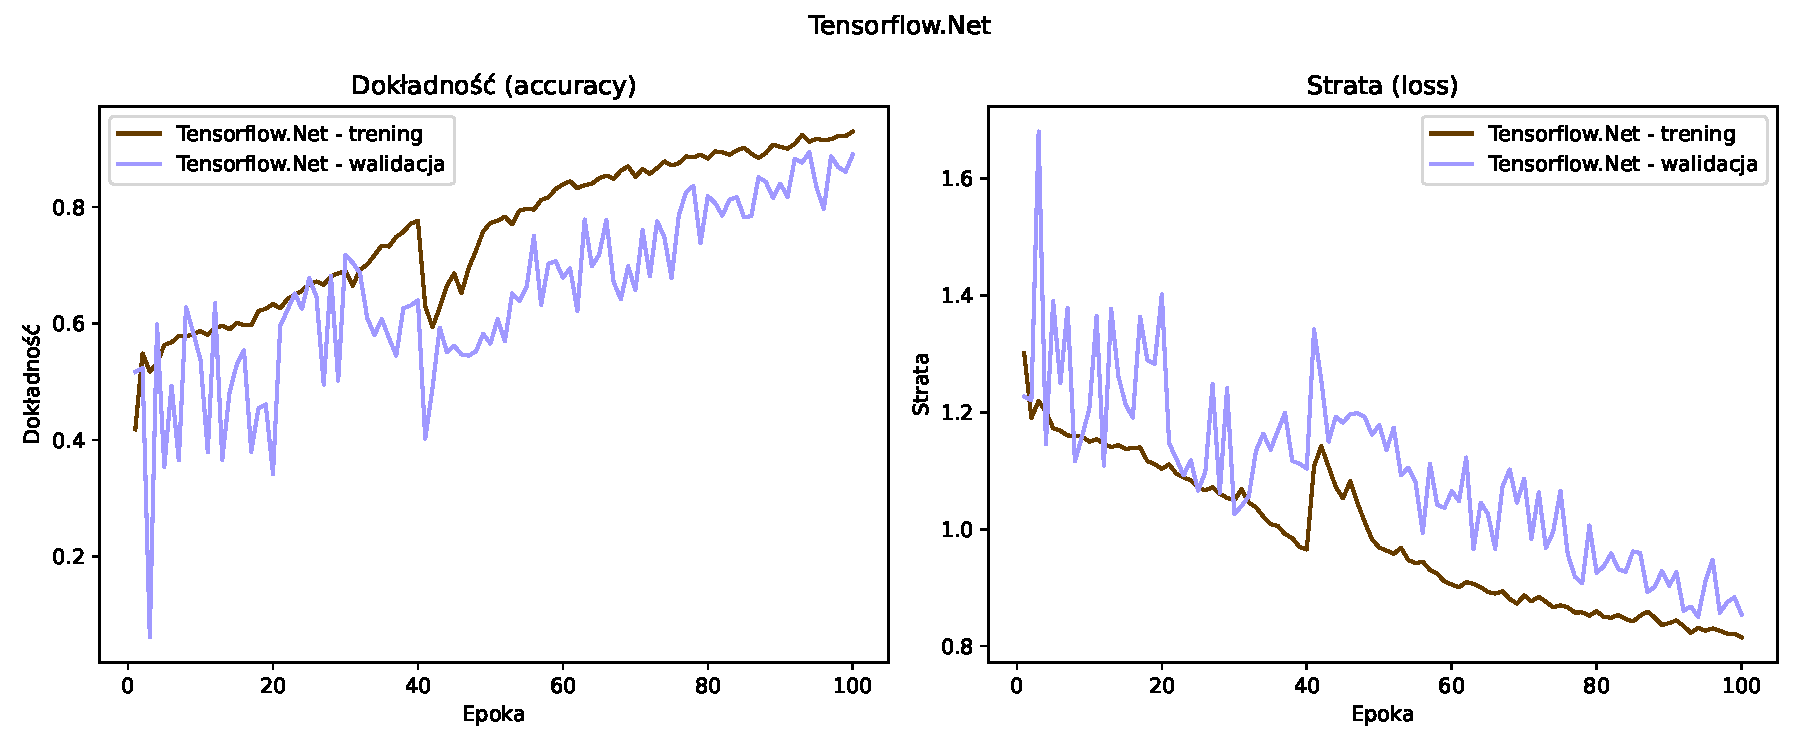
\includegraphics[width=\textwidth]{plot-tensorflownet-training-overview}
  \caption[Wykresy statystyk modelu Tensorflow.NET w~trakcie uczenia]{Wykresy dokładności (\emph{accuracy}) oraz straty (\emph{loss}) dla danych testowych i~walidacyjnych modelu \emph{Tensorflow.NET} w~trakcie uczenia}
  \label{fig:plot-tensorflownet-training-overview}
\end{figure}

Jak widać na wykresie, dokładność oraz strata walidacyjna są bardzo chaotyczne i~mają wiele dużych skoków i~spadków w~trakcie uczenia, gdzie z~kolei dokładność oraz strata treningowa są znacznie bardziej stabilne mimo jednego większego skoku w~środkowej fazie uczenia.
Mimo wszystko zarówno na zbiorze treningowym, jak i~walidacyjnym dokładność rośnie, a~strata maleje, co wskazuje na to, że model się poprawnie uczy.

Tak wytrenowany model (który znajduje się wraz z~kodem źródłowym i~wynikami w~repozytorium) został następnie przetestowany na zbiorze testowym, który nie został użyty w~procesie uczenia, a~więc sieć widziała pojawiające się tam obrazy po raz pierwszy.

Maksymalna dokładność modelu na zbiorze testowym wyniosła $91.2\%$, a~na zbiorze walidacyjnym $89.4\%$, co jest wynikiem pozwalającym na rozważenie wykorzystania modelu w~praktyce, choć nadal nie idealnym.
Jest to wynik tym bardziej pozytywny biorąc pod uwagę, że wyszkolona sieć uzyskała dokładność na zbiorze testowym $85.9\%$, a~więc stosunkowo wysoką.

\section{Porównanie wyników}

W pierwszej kolejności warto zacząć od porównania wyników uzyskanych przez projekty opierające się o~framework \emph{ML.NET}, nazwane \emph{ML.NET Custom} (dalej \emph{MLCustom}) oraz \emph{ML.NET Model Builder} (dalej \emph{MLBuilder}), czyli kolejno projekt oparty o~własny kod wykorzystujący API biblioteki oraz projekt wykorzystujący narzędzie wbudowane w~Visual Studio.
Wykres zestawienia zmiany dokładności modelu w~trakcie uczenia dla zbioru treningowego oraz dla zbioru walidacyjnego został przedstawiony na \hyperref[fig:plot-mlnet-custom-vs-mlnet-model-builder]{rysunku \ref*{fig:plot-mlnet-custom-vs-mlnet-model-builder}}.

\begin{figure}[ht]
  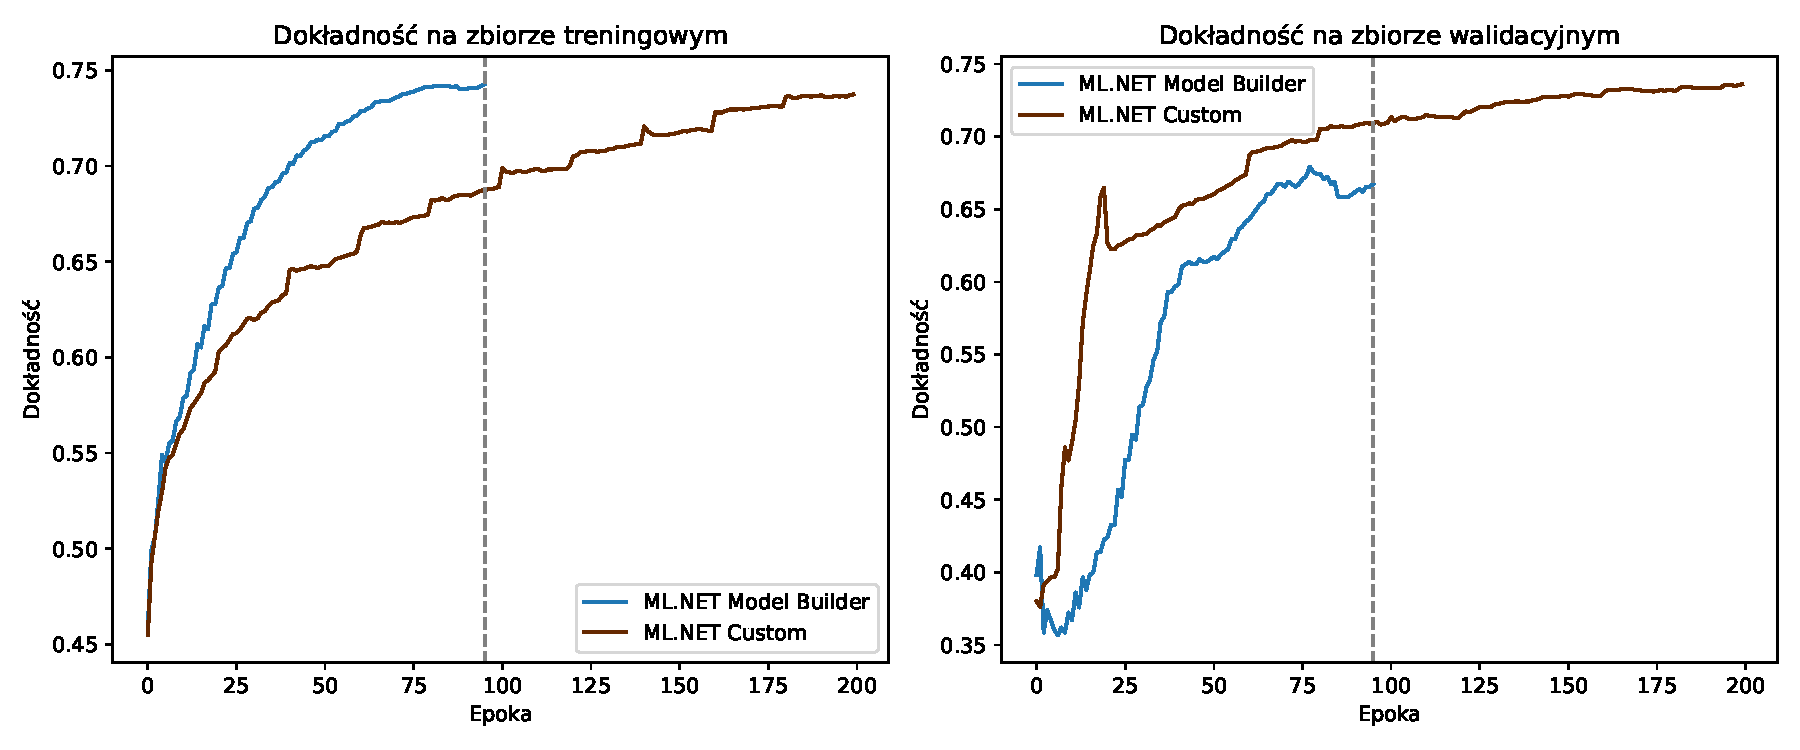
\includegraphics[width=\textwidth]{plot-mlnet-custom-vs-mlnet-model-builder}
  \caption[Porównanie dokładności oraz straty modeli ML.NET Custom oraz ML.NET Model Builder]{Porównanie dokładności (\emph{accuracy}) oraz straty (\emph{loss}) na zbiorze treningowym i~walidacyjnym modeli z~projektów \emph{ML.NET Custom} oraz \emph{ML.NET Model Builder}}
  \label{fig:plot-mlnet-custom-vs-mlnet-model-builder}
\end{figure}

Pierwszym zauważalną różnicą jest fakt, że model \emph{MLCustom} uczony był aż $200$ epok, gdzie model \emph{MLBuilder} jedynie $95$.
U tego drugiego jednak krzywa dokładności na zbiorze testowym rosła znacznie szybciej i~zdążyła osiągnąć prawdopodobny punkt maksymalny, gdzie \emph{MLCustom} tego samego punktu nie osiągnął nawet na koniec swojego uczenia dwukrotnie później.

Sytuacja ma się jednak nieco odwrotnie i~komplikuje wyciągnięcie jednoznacznych wniosków w~przypadku dokładności na zbiorze walidacyjnym.
Na tym wykresie bowiem \emph{MLCustom} od samego początku miał wyższą skuteczność niż \emph{MLBuilder} i~utrzymywał tę przewagę do końca procesu uczenia tego drugiego, później nawet ją podwyższając.
Kształt krzywej dokładności na zbiorze walidacyjnym w~przypadku obu projektów wygląda bardzo podobnie, gdzie uczenie zwalniało po osiągnięciu dokładności mniej więcej $0.62$ z~późniejszym powolnym wzrostem.

Należy do porównania dodać także dokładność modeli na zbiorze testowym, który nie został użyty w~procesie uczenia, w~którym MLCustom osiągnął zaledwie $45.3\%$, a~MLBuilder $70.6\%$ znacznie bardziej zbliżone do dokładności na zbiorze walidacyjnym.
Sugerować to może, że dokładność na zbiorze walidacyjnym projektu \emph{MLCustom} wynikała z~czynników losowych lub błędnie dobranych parametrów uczenia, przez co nie współgrała z~dokładnością na zbiorze treningowymi ani nie odpowiadała w~rzeczywistości dokładności na zbiorze testowym.

Można więc wnioskować, że automatyczne dobieranie parametrów uczenia przez \emph{MLBuilder} pozwoliło na uzyskanie lepszych wyników niż własnoręczne dobieranie parametrów przez \emph{MLCustom}.

Następnie możemy porównać lepszy z~pary projektów bazujących na ML.NET z~projektem niestandardowego modelu głębokiej konwolucyjnej sieci neuronowej zbudowanej i~wyszkolonej za pomocą biblioteki \emph{TensorFlow.NET}.
Tutaj pojawiają się także istotne różnice strukturalne, gdzie projekt \emph{MLBuilder} bazuje na uczeniu transferowanym z~wykorzystaniem gotowych modeli sieci neuronowych, a~projekt \emph{TensorFlow.NET} na własnoręcznie zbudowanej sieci konwolucyjnej dostosowanej do zadań klasyfikacyjnych na obrazach rezonansu magnetycznego mózgu.
Wykres zestawienia zmiany dokładności modelu w~trakcie uczenia dla zbioru treningowego oraz dla zbioru walidacyjnego został przedstawiony na \hyperref[fig:plot-mlnet-model-builder-vs-tensorflownet]{rysunku \ref*{fig:plot-mlnet-model-builder-vs-tensorflownet}}.

\begin{figure}[ht]
  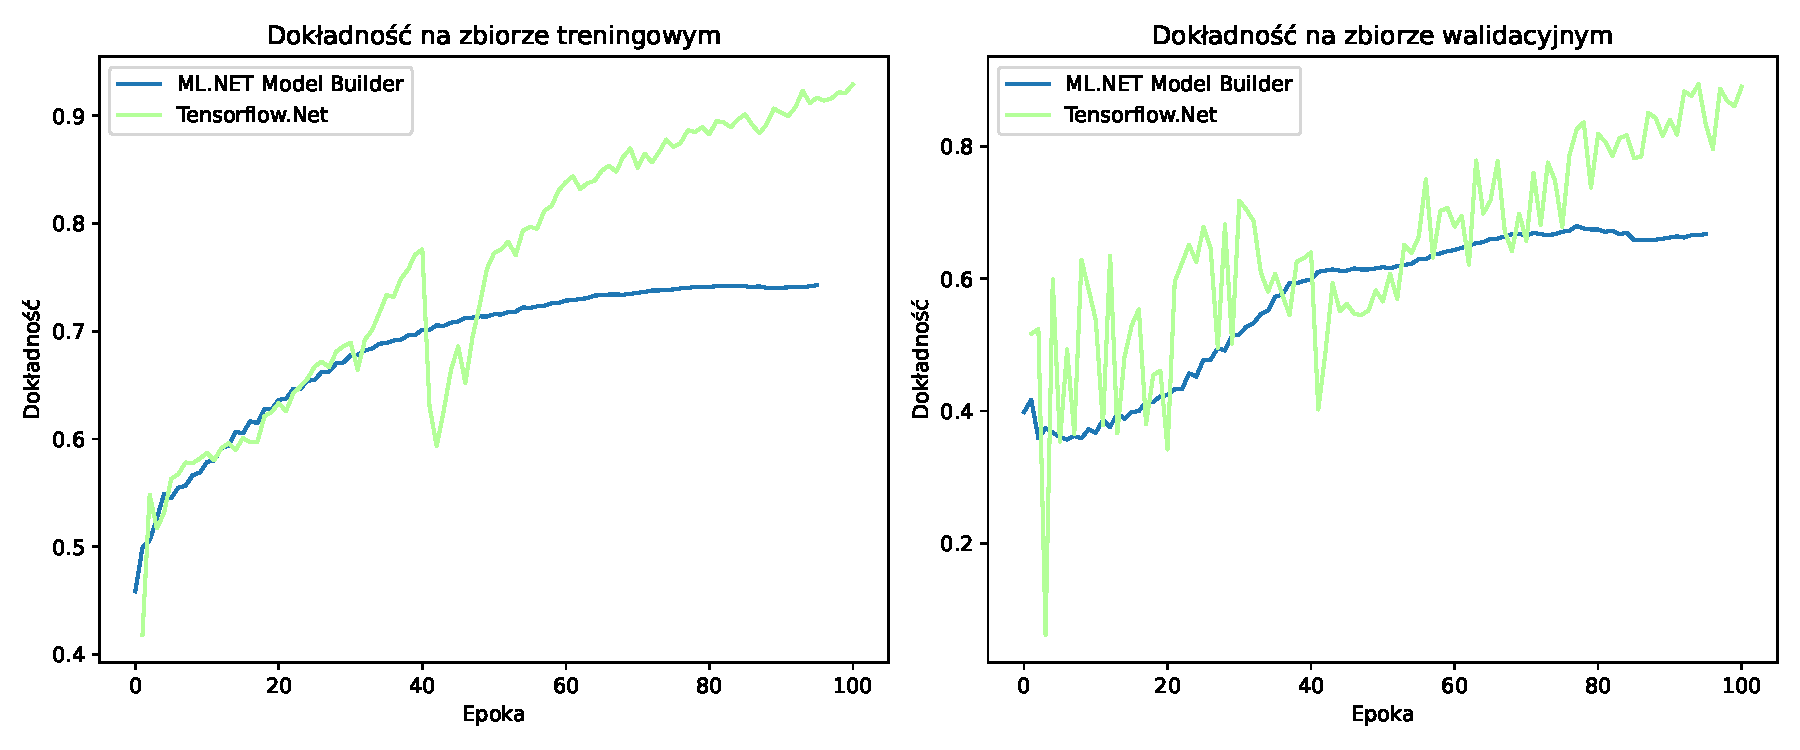
\includegraphics[width=\textwidth]{plot-mlnet-model-builder-vs-tensorflownet}
  \caption[Porównanie dokładności oraz straty modeli ML.NET Model Builder oraz Tensorflow.NET]{Porównanie dokładności (\emph{accuracy}) oraz straty (\emph{loss}) na zbiorze treningowym i~walidacyjnym modeli z~projektów \emph{ML.NET Model Builder} oraz \emph{Tensorflow.NET}}
  \label{fig:plot-mlnet-model-builder-vs-tensorflownet}
\end{figure}

Na wykresie wyraźnie widać, że model \emph{Tensorflow.NET} osiągnął znacznie wyższą dokładność zarówno na zbiorze treningowym, jak i~w zbiorze walidacyjnym.
Proces uczenia był zdecydowanie mniej stabilny, gdzie krzywa dokładności \emph{MLBuilder} jest bardzo gładka z~niewielkimi zmianami prawdopodobnie wynikającymi z~niskiej wartości współczynnika uczenia, gdzie krzywa dokładności drugiego projektu jest chaotyczna i~ma wiele dużych skoków i~spadków w~trakcie uczenia.
Do epoki mniej więcej $30$ lub $40$ modele radziły sobie porównywalnie, jednak, gdzie \emph{MLBuilder} zaczął zwalniać, tam \emph{Tensorflow.NET} nadal wyraźnie poprawiał swoje działanie.

Warto zauważyć, że czas mimo zbliżonej ilości epok uczenia, rzeczywisty czas ich przeprowadzenia był diametralnie różny.
Oba modele szkolone były na tym samym sprzęcie, wykorzystując do niego ten sam procesor graficzny \emph{NVIDIA GeForce GTX 1060 Max-Q}.
Jak pokazują logi z~uczenia w~przypadku \emph{MLBuilder} (które również zawarte są w~repozytorium), całość szkolenia modelu zajęła nieco ponad $270$ sekund, to jest $4.5$ minuty.
Natomiast jednokrotne przeszkolenie modelu \emph{Tensorflow.NET} zajęło ponad 3~godziny, czyli prawie 3~rzędy wielkości więcej czasu.
Różnica ta wynika przede wszystkim z~faktu, że w~przypadku \emph{MLBuilder} wykorzystywane jest uczenie transferowane, gdzie już duży, wyszkolony model sieci neuronowej jest tylko ``dostrajany'' za pomocą danych treningowych do rozwiązania konkretnego problemu, co znacznie zmniejsza ilość parametrów sieci do wyszkolenia.
W przypadku \emph{Tensorflow.NET} natomiast sieć jest bardzo duża jest budowana od podstaw i~musi nauczyć się własną ogromna ilość parametrów od zera, co znacznie wydłuża czas uczenia.

Nie zmienia to faktu, że kluczowym czynnikiem porównania jest finalna skuteczność powstałych sieci neuronowych.
W tym przypadku model \emph{Tensorflow.NET} uzyskał dokładność na zbiorze treningowym $91.2\%$, a~na zbiorze walidacyjnym $89.4\%$, co w~porównaniu z~rezultatem \emph{MLBuilder} $74.0\%$ na zbiorze treningowym i~$67.9\%$ na zbiorze walidacyjnym jest znacznie lepszym o~około $0.2$, co przy takich wartościach jest znaczącą różnicą.
Dodatkowo ten pierwszy model uzyskał dokładność na zbiorze testowym $85.9\%$, a~ten drugi $70.6\%$, co jest wynikiem znacznie lepszym.

\begin{table}[ht]
  \centering
  \begin{tabular}{|l|r|r|r|r|}
    \hline
                         & \multicolumn{2}{c|}{Zbiór treningowy}                                          & \multicolumn{2}{c|}{Zbiór walidacyjny}                      \\
    \cline{2-5}
                         & \multicolumn{1}{|c|}{Accuracy}        & \multicolumn{1}{|c|}{Loss}             & \multicolumn{1}{|c|}{Accuracy} & \multicolumn{1}{|c|}{Loss} \\
    \hline
    ML.NET Custom        & 0.7373874                             & 0.6378530                              & 0.7359702                      & 0.6511808                  \\
    ML.NET Model Builder & 0.7401715                             & 0.6036751                              & 0.6793103                      & 0.7503802                  \\
    Tensorflow.NET       & 0.9118868                             & 0.8311445                              & 0.8935547                      & 0.8501284                  \\
    \hline
  \end{tabular}
  \caption[Porównanie dokładności oraz straty modeli na zbiorze treningowym i~walidacyjnym]{Porównanie dokładności (\emph{accuracy}) oraz straty (\emph{loss}) modeli na zbiorze treningowym i~walidacyjnym w~epokach szkolenia najlepszych względem na dokładności walidacyjnej}
  \label{tab:train_validation_metric_comparison}
\end{table}

Wszystkie wyniki dotyczące dokładności i~straty modeli w~trakcie uczenia na zbiorze testowym oraz walidacyjnym zostały przedstawione w~\hyperref[tab:train_validation_metric_comparison]{tabeli \ref*{tab:train_validation_metric_comparison}}.

Najistotniejszą statystyką jednak jest dokładność modeli na zbiorze testowym, który nie został użyty w~procesie uczenia, a~więc sieć widziała pojawiające się tam obrazy po raz pierwszy.
Ona dopiero sugeruje, jak model może sprawować się w~praktyce na rzeczywistych, nowych obrazach.
Wyniki te zostały przedstawione w~\hyperref[tab:test_accuracy_comparison]{tabeli \ref*{tab:test_accuracy_comparison}}.

\begin{table}[ht]
  \centering
  \begin{tabular}{|l|r|}
    \hline
                         & \multicolumn{1}{|c|}{Accuracy} \\
    \hline
    ML.NET Custom        & 0.45269742                     \\
    ML.NET Model Builder & 0.70602033                     \\
    Tensorflow.NET       & 0.85926505                     \\
    \hline
  \end{tabular}
  \caption[Porównanie dokładności modeli na tym samym zbiorze testowym]{Porównanie dokładności (\emph{accuracy}) modeli na tym samym zbiorze testowym}
  \label{tab:test_accuracy_comparison}
\end{table}

Jak widać, model \emph{Tensorflow.NET} uzyskał najwyższą dokładność na zbiorze testowym.
Poprawne wykrycie poziomu demencji oraz choroby Alzheimera z~obrazu rezonansu magnetycznego mózgu na poziomie $85.9\%$ jest wynikiem, który pozwala na rozważenie wykorzystania modelu w~praktyce.
Do celów diagnostycznych więc utworzenie niestandardowego modelu głębokiej sieci neuronowej z~wykorzystaniem biblioteki \emph{Tensorflow.NET} dostosowanego do wykorzystania w~analizie obrazów jest najlepszym dostępnym rozwiązaniem z~tych przeanalizowanych w~tej pracy.

\section{Wykorzystanie modelu w~aplikacji z~użyciem biblioteki ML.NET}

Istotnym faktem do zaznaczenia jako swoista adnotacja do wyników analizy jest to, że tak na prawdę przeprowadzone badanie i~wyniki z~niego wyciągnięte w~rzeczywistości przedstawia porównanie użytych bibliotek jako narzędzia do samego projektowania i~uczenia głębokich sieci neuronowych dla detekcji choroby Alzheimera.
Natomiast pominięty całkowicie został aspekt późniejszego wykorzystania powstałych modeli.

Faktycznie jak pokazały wyniki, nauczenie modelu przy pomocy biblioteki \emph{Tensorflow.NET} pozwala na uzyskanie lepszych wyników.
Dzieje się tak przede wszystkim dzięki możliwości zbudowania dużo bardziej wyspecjalizowanej sieci neuronowej oraz bezpośrednie wykorzystanie bibliotek \emph{TensorFlow} oraz \emph{Keras}, bardzo popularnych, dobrze rozwiniętych i~bardzo wydajnych.

\emph{Tensorflow.NET} jednak przez swoje podobieństwo w~sposobie pisania kodu do języka \emph{Python} staje się bardzo nieczytelny w~otoczeniu kodu środowiska \emph{.NET} i~języka C\#, jest trudny do faktycznego wykorzystania w~projekcie.
Jednak możliwe jest wygenerowanie wyszkolonego modelu do formatu \emph{SavedModel}, \emph{ONNX} lub innego wspieranego oraz jego późniejsze wczytanie w~projekcie używając biblioteki \emph{ML.NET}.
Co więcej, wczytać można model wyszkolony z~użyciem dowolnego narzędzia, chociażby samej biblioteki \emph{Keras} w~języku Python.

Tak wyszkolony model ma wszystkie zalety szkolenia z~użyciem \emph{TensorFlow} i~identyczną skuteczność, ale dzięki wczytaniu i~użyciu biblioteki \emph{ML.NET} znacznie lepiej komponuje się z~rzeczywistymi projektami środowiska \emph{.NET} i~języka \emph{C\#}, między innymi w~oprogramowaniach szpitalnych czy szerzej w~medycynie.

Takie wykorzystanie wczytanego modelu przedstawione zostało w~projekcie \lstinline{MLModel_ConsoleApp} oraz \lstinline{MLModel_WebApi} w~solucji \lstinline{VisualStudioModelBuilder.sln} w~repozytorium opisanym w~\hyperref[sec:source-code]{sekcji \ref*{sec:source-code}}.
W nim wczytywany jest model wygenerowany przez \emph{ML.NET} we własnym formacie, jednak nic nie stoi na przeszkodzie zamiast niego wczytać model wyszkolony z~zewnątrz przez \emph{TensorFlow} lub inne narzędzie, co można osiągnąć wywołaniem metody \lstinline{ApplyOnnxModel} wczytującej model formatu ONNX.
